
\section{Historical fundamentals}


\subsection{Renaissance}

The Renaissance is a historical period from 14th to 17th century, which started as a cultural movement in Italy in the Late Medieval period and later spread to the rest of Europe. This period is considered as the bridge between Middle Ages and Modern History. Even though the renaissance had a major impact all over Europe, the spread of its principles was not made in an uniform fashion. The word Renaissance, litterally meaning "Rebirth" in French, first appears in English in the 1830s.
The Renaissance is mostly known for the cultural revival of the principles developed in the ancient Greece and Roman Empire. This revival brought a gradual a widespread educational reform.
Renaissance had a major role  in politics, its principles being the base of the conventions of diplomacy. In science, the renaissance brought an increased reliance on observation, rather than superstition.
Even though the renaissance had a major impact in all aspects of life between 14th and 17th century, this historical period is mostly known for the impact it had on arts. The most famous examples are the artistic developments and contributions of such polymaths as Leonardo da Vinci and Michelangelo, who inspired the term "Renaissance man".
The Renaissance started in Italy in the 14th century, under the patronage if powerful, dominant families as Medici. The Fall of the Constantinople at the hands of the Ottoman Turks started a migration of Greek scholars towards west. This scholars brought with them the wisdom and knowledge of the ancient Greece and Rome and spread it though the Italian peninsula, in all the major city states, such as Florence, Venice, Genoa, Bologna, Milan and finally Rome, during the Renaissance papacy.
Renaissance influence was felt in literature, philosophy, art, music, politics, science, religion, and other aspects of intellectual inquiry. Renaissance scholars employed the humanist method in study, and searched for realism and human emotion in art.
Renaissance could be considered as an attempt to study and improve the secular and worldly, both through the revival of ancient ideas and principles, and though new approaches to thoughts.
Another major influence of the Renaissance was felt in the economy. One of the best example could be the banking system pioneered by the Medici family in Florence. While the great states of Europe, France and Spain were absolutist monarchies and ma other states were under direct papal control, the independent city republics of the Italian peninsula took over the capitalist principles developed on the monastic estates, and set off a vast unprecedented commercial revolution and financed the Renaissance.

Renaissance Architecture, is the architecture of the period between 15th and 17th century. This period is characterized by a conscious revival and development of ancient Greek and Roman thought and material culture.
Stylistically, Renaissance architecture followed Gothic architecture and was succeeded by Baroque architecture.

"Renaissance style places emphasis on symmetry, proportion, geometry and the regularity of parts as they are demonstrated in the architecture of classical antiquity and in particular ancient Roman architecture, of which many examples remained. Orderly arrangements of columns, pilasters and lintels, as well as the use of semicircular arches, hemispherical domes, niches and aedicules replaced the more complex proportional systems and irregular profiles of medieval buildings."
Renaissance in Germany
Renaissance arrival in Germany and the Low Countries coincided with the development of the printing press (ca. 1450) and was inspired first by German philosophers and artists such as Albrecht Dürer and Johannes Reuchlin who visited Italy.
In the early Protestant regions of the country, the humanism became closely related with the religious turmoil caused by the Protestant Reformation. Various aspects of this turmoil were frequently depicted in the art and the literature from this period. However, the gothic style and medieval scholastic philosophy remained dominant until the turn of the 16th century. With the rise to power of the Emperor Maximilian I of Habsburg (1493-1519), renaissance became the main trend in the land. The emperor was the first truly Renaissance monarch of the Holy Roman Empire, later known as Holy Empire of the German Nation.
One important early example of renaissance architecture is Landshut Residence. In 1536 Louis X, Duke of Bavaria laid the foundation stone for a new residence in the inner city of Landshut. It was the beginning of German Renaissance style under the architect Bernhard Zwitzel from Augsburg; this palace is today known as the "German building". During a journey to Italy, the duke got inspiration for an additional building, the so called "Italian building", which was constructed from 1537 to 1543 in Italian renaissance style.
Another important example of renaissance architecture in Germany is the Augsburg Town Hall. The Town Hall of Augsburg is the administrative centre of Augsburg, Bavaria, Germany, and one of the most significant secular buildings Convention for the Protection of Cultural Property in the Event of Armed Conflict.
The largest renaissance church north of the Alps is St. Michael's Church in Munich. St. Michael's Church is a Jesuit church built between 1583 and 1597 by Wiliam V, Duke of Bavaria. The style in which this church was built will have an enormous influence on Southern German early Baroque architecture. This church was built as the spiritual center for the Counter Reformation. In order to build the church and the adjoining collage, Duke William had to pull down 87 houses, ignoring the protests of the citizens.
Weser Renaissance is a style formed around river Weser in central Germany. The style is very well preserved in the towns and cities of that region. 
Between the start of the Reformation and the Thirty Years War, the Weser region experienced a construction boom, in which the Weser, playing a significant role in the communication of both trade and ideas, merely defined the north-south extent of a cultural region that stretched westwards to the city of Osnabrück and eastwards as far as Wolfsburg.
Castles, manor houses, town halls, residential dwellings and religious buildings of the Renaissance period have been preserved in unusually high density, because the economy of the region recovered only slowly from the consequences of the Thirty Years War and the means were not available for a baroque transformation such as that which occured to a degree in South Germany.

Characteristics:
https://www.youtube.com/watch?v=tVmVnW4rL4s


The Pellerhaus
The Pellerhaus on Egidienplatz 23 in Nuremberg was once considered one of the most magnificent examples of a town house of the German Renaissance achitecture.
The house was commissioned by Martin Peller in 1602 and remained in the possession of the Peller family until 1828. 

During the next 100 years the house changes hands several times until 1929 when is bought by the city of Nuremberg under the mayor Herman Luppe. The acquisition of the house by the city assured a proper maintenance of this historical landmark.
Between 1931 and 1934 the city starts a reconstruction program for Pellerhaus, restoring to the old grandeur the yard and the rear facade. The detailed plans of the rear facade, drawn for this project survive until today.
On January 2nd, 1945, Pellerhaus was destroyed in an ally bombing. In fact a huge part of the city was transformed into a leveled surface by bombing and debris removal. 
The elegant and dignified image of Egidienplatz, is not distorted by the flat-roof building of the City Library built between 1955 and 1957. The new reconstruction project is launched in 1955, only this time it was decided to restore to its former glory only the ground floor. The rest of the building will serve only a pure functional role and serve as a library for many years.
In 2005 a new initiative was launched, to help with the reconstruction of Pellerhaus. This project is still active today.\\


See Wikipedia: \url{http://en.wikipedia.org/wiki/The_Renaissance} 

\subsection{Architects}

A detailed biography of the architects can be found in the Appendix (\ref{appendix_pellerhaus_architects}).

\subsection{Pellerhaus}

The association Altstadtfreunde e.V. created a flyer \parencite{afWiederaufbauDesPellerhofes} where a wonderful description was written that has been translated by the author from German:

\blockquote{
	Before destruction, the Pellerhaus was one of the main sights of Nuremberg. The architecture seems to be the most honorable performance of the local art of construction. Its inner court was considered the probably most beautiful arcade court.\\
	As the city descended into shatters in 1945, there were only a few remains of the Pellerhaus. The front-facing house was rebuilt in a modern form 1957 on top of the reconstructed hall. An enourmous effort was done by complementing the courtyard, it was discontinued 1959, though.\\
	Not until 2005, 60 years after the destruction, the Altstadtfreunde took the initiative to continue the former abandoned construction of side wing and rear house facade.\\
	With the accurate documentation of the pre-war level it is possible to do those court additions with extraordinary accuracy. October 2008 layed the foundation block of building the courtyard completely via donations.\\
	Since then with the well corner, side wings and eastern backyard gallery crucial parts have been able to get restored from the old building.\\
	With your donation or by purchasing a symbolic block of stone you can help to make one of the greatest achievements of German Renaissance in its historic state come alive.\\
	At the time when the merchant Martin Peller started with building his house in 1602, he also layed the foundation block to what later entered as the most magnificient bourgeois house into the history of art. The notion of building an arcade court was not new in Nuremberg. There have been hundreds of gallery courts in the city. Many of them with tracery breastwork made of stone. Though, the Pellerish courtyard bested everything that has been know at that time:\\
	On the two long sides it was flanked by noble three-story arcades, with a clear and symmetric structure, though with a rich and filigreed ornamentation. While skimming along it, ultimately the show façade caught the eye with a glorious gable. Seldom one can find forms of the italian renaissance merged with local sensuous enjoyment in such a happy way. Antique style pillars accompany the individual floors, obelisks stretch up into the sky and still the appearance was entirely different than in Italy. The Pellerhof, as a Middle European counterpart to the wonderful arcade courts of Italy, is an indispensable part of european architecture .\\
}



\begin{figure}[h]
	\centering
	\begin{subfigure}[b]{0.3\textwidth}
		\centering
		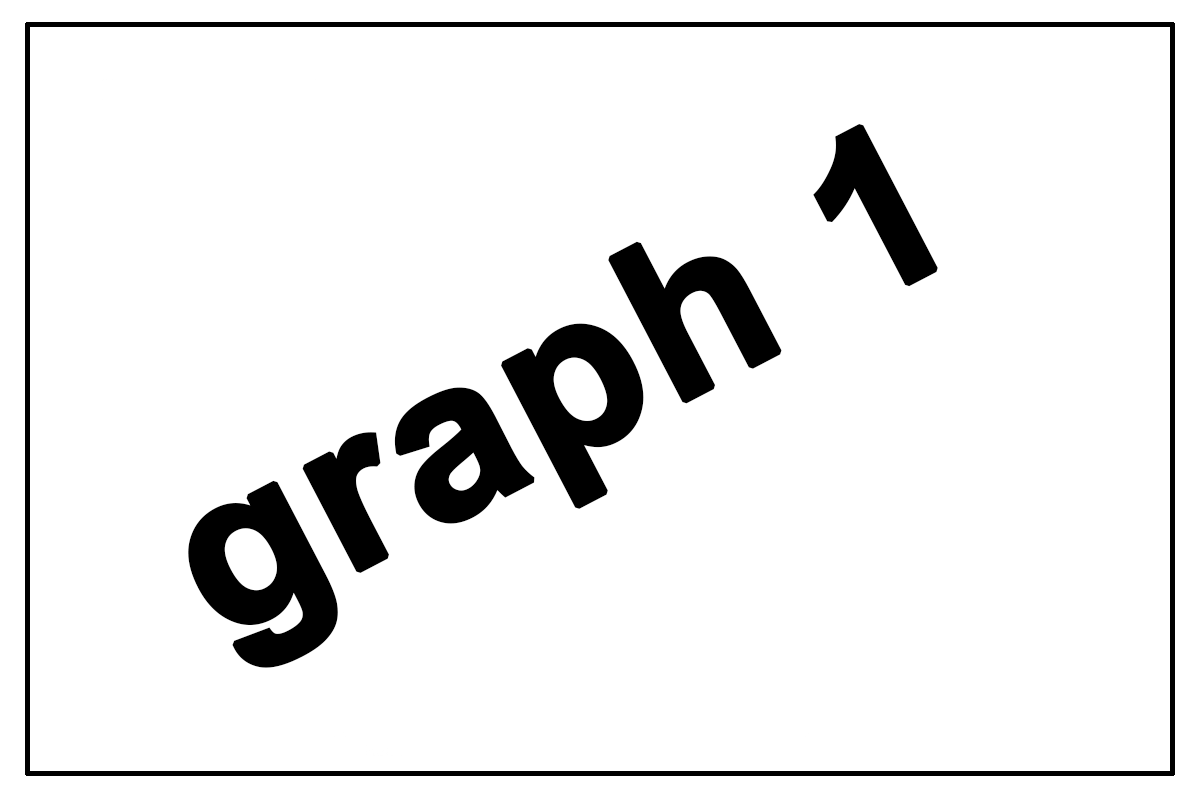
\includegraphics[width=\textwidth]{graph1.png}
		\caption{$before 1945$}
		\label{fig:pellerhaus_historic}
	\end{subfigure}
	\hfill
	\begin{subfigure}[b]{0.3\textwidth}
		\centering
		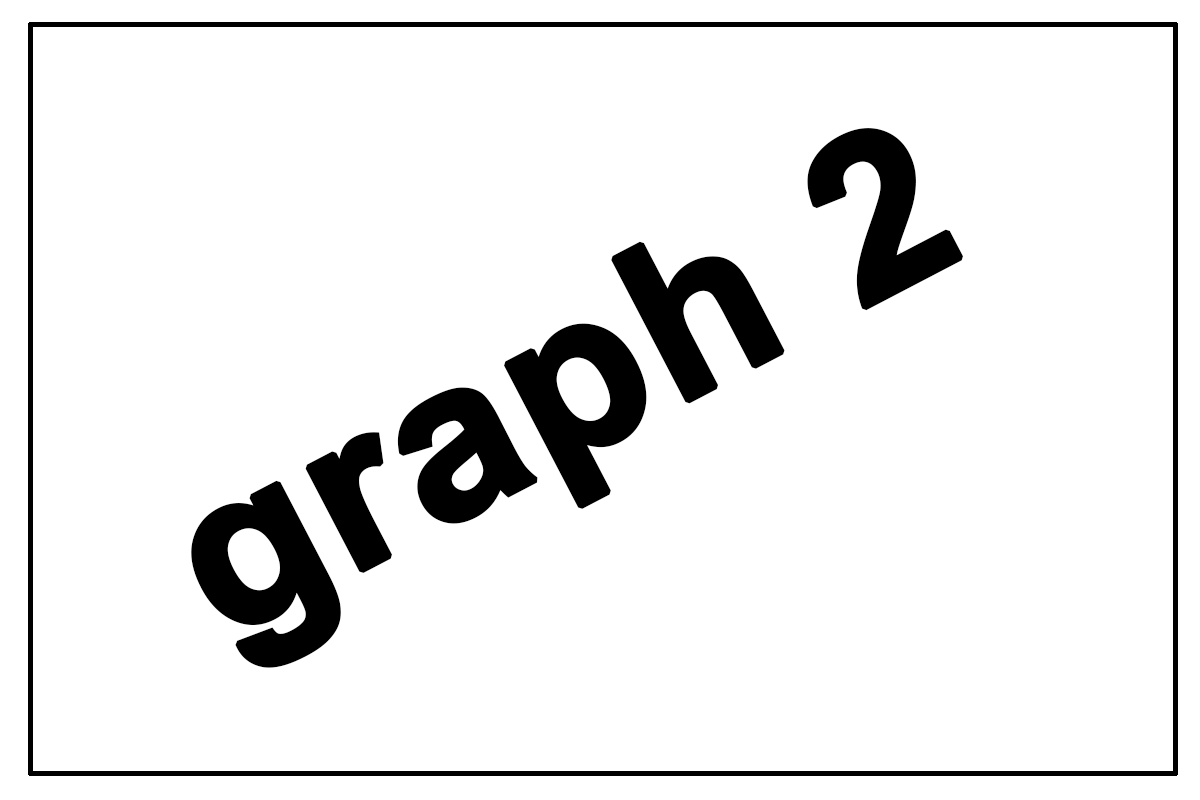
\includegraphics[width=\textwidth]{graph2.png}
		\caption{$Pellerhaus 1945$}
		\label{fig:pellerhaus_destructed}
	\end{subfigure}
	\hfill
	\begin{subfigure}[b]{0.3\textwidth}
		\centering
		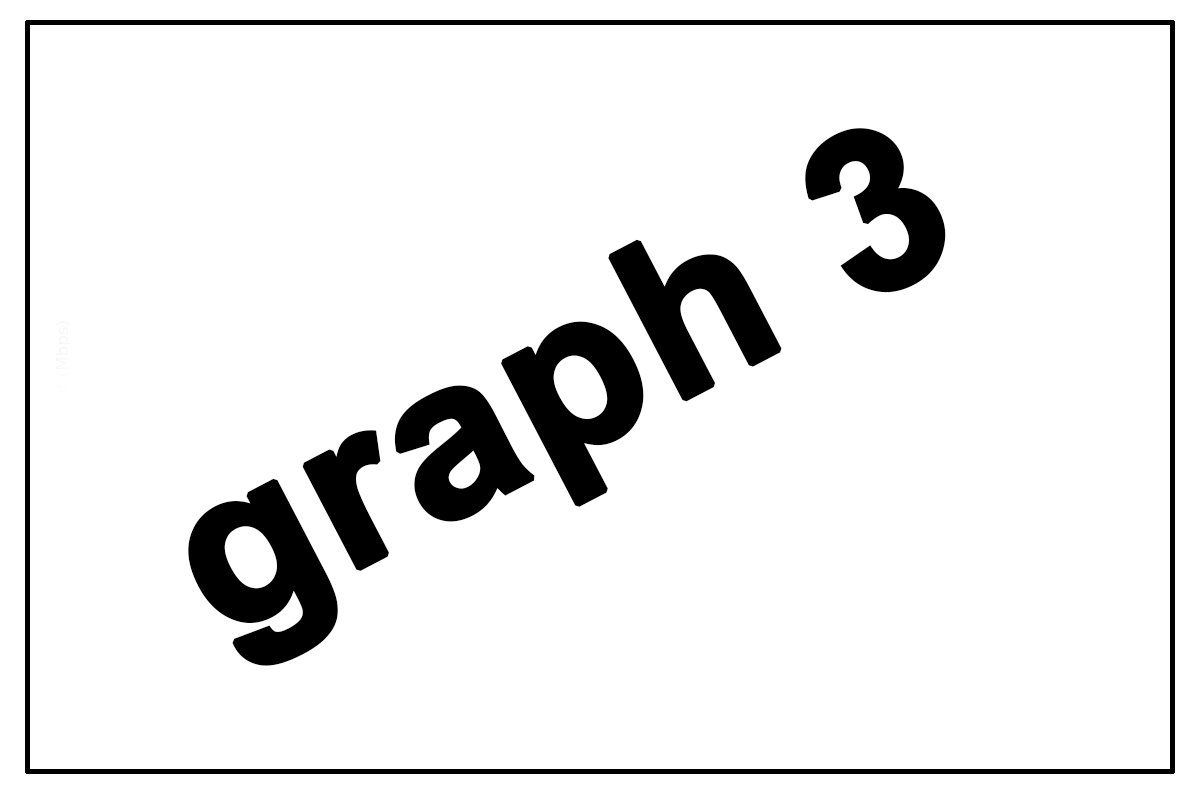
\includegraphics[width=\textwidth]{graph3.png}
		\caption{$after 1945$}
		\label{fig:pellerhaus_modern}
	\end{subfigure}
	\caption{The Evolution of the Pellerhaus}
	\label{fig:pellerhaus_states}
\end{figure}

First reconstruction was finished in 1934.
Destruction in 1945.
1955 beginning of new reconstruction.
1955-1957 reconstruction of the base floor finished, but destruction of the upper floors (storey heights also differ from the original).
1960 End of all reconstructions, though people realized that a full reconstruction might happen
1972/73 Building a secondary school on top of the back-facing house area pretty much killed every hope of reconstruction of the Pellerhaus.
The Pellerhof has groined vault.\parencite{afPellerhausMagazin01} \\

The Pellerhaus was bought by the Major of Nuremberg in the year 1929. Reconstruction was estimated to need a budget of a Martin Peller to succeed. It was a real mess. But the city felt responsible to finance the reconstruction at that time and fundamentally restored it from 1931 to 1934. The red facades have been cleared up and new stone details have been redone by hand. The were really careful to keep all of the small details and not to recreate the house according to a recent art period. The Pellerhaus was saved. Ten years later, it was hit by bombs. Though, the former restoration is incredible worthy today. Hundreds of plans and photos document every detail of its facade. Without that documentation a reconstruction would have been extremely difficult today.
Why wasn't the Pellerhaus reconstructed?
After the Second World War it was important to find room for e.g. the city archive and a library. It was almost decided to completely embed the Pellerhaus into the library which was build to the right of it. But there was a certain force within the city that didn't allow that. So in the end, the old style Pellerhaus was combined with a new style to allow experiencing the old state a little.\parencite{afPellerhausMagazin02} \\

Right to the Pellerhaus there was a library built in 1955. An old arc was destroyed which was senseless. Only some column bases and capitals were still laying in the inner courtyard and were ready to be build into the southern part of the court. So, all six arcs, the little passage next to the front-facing house and the adjacent facade part of the northern court facade needed to be recreated.
The build process was mainly based on photos and the remains of the western side. Measurements have been extracted by examining the remains. Also profiles and design of capitals and ending stones. Overall Forms were reconstruced with the help of historic photos. New constructions were needed for the differing tracery of balustrade areas. It was a stroke of luck that the historic documentation of the house is extensive. This helped even with differences of geometric correct constructions with the new build. Also the Chörleins are documented well enough to allow for a reconstruction. For example, there is a massively wrong ornamentation of Chörleins at window lintels, sockets, and volutes when comparing the rebuild from 1950 with the original. On the contrary, we are much closer at the renaissance original with our new build.
We can proudly say that with our restored state the two time layers 1605/07 and 1957/59 form a harmonic unit.
From April 2013 we moved newly produced stone blocks and a fully donated arc in the pellerhaus. Once again, we noticed the reckless deviation of any regularity. All of the six arcs have different spans and the alignment of the arcarde row is not straight, but has been – in its old parts – slightly bulged out. Though, this might be due to the bombing destruction, just as the fact that the arc row
doesn't continue horizontally but considerably descends from the front-facing house into the courtyard.
The facades of the buildings in Nuremberg have been painted red with white rectangles some times. The reason for this was that the look of mined stones varied quite a lot. So by painting them the houses had a united look. This color is also called the „Nürnberger Rot“ (Terra Norimbergensis rubra), because it is looking like the local sand stone and the color powder is coming from the rural area of Nuremberg. Unfortunately only a few color remains are left until the reconstruction but it is enough to prove the colorfulness of the facade. After finishing the reconstruction in the courtyard repainting the facades in the „Nürnberger Rot“ would be the right decision.\parencite{afPellerhausMagazin03} \\


Nuremberg had substantial achievements in the field of architecture around 1600. Significant public and private buildings have been built between the end of the Second Margrave War and the beginning of the Thirty Years' War.
The first big construction project after the end of the war against Albrecht Alcibiades was the fortification of the defense structures. During 1556-1564, the wall ring was improved and the towers of the five main gates (Laufer Tor, Spittlertor, Frauentor, Neutor, Vestnertor) were surrounded by a stone wall. This was inspired by the towers of Castle Sforza in Milano, Italy.

Additional important public buildings were realized by the (royal adviser?) city builder Jacob Wolff der Ältere (1596-1612) and his son Jacob Wolff der Jüngere (1612-1620) during that time. The most important ones have been the construction of the Fleischbrücke inspired by the Ponte Rialto in Venedig (after 1596), the Wöhrder Torbastei (1613/1614), the master builders' house on the Peunt (1615) and especially the city hall, which was inspired by late renaissance style palaces in Italy (1616-1622).

Besides the public buildings there were created several considerable private structures around 1600. They mostly haven't been commissioned by patricians but rich merchants. The most important ones have been the Toplerhaus (1590), the Fembohaus (1591) and the Pellerhaus (1602-1607).
At the same time many manors in the land domain of Nuremberg have been rebuilt in the following decades after the Second Margrave War.

\parencite[translated from German]{bookAcademiaNorica}




\section{3D Panorama}

In 2D words, a panorama is an image.

\begin{figure}[h]
	\centering
	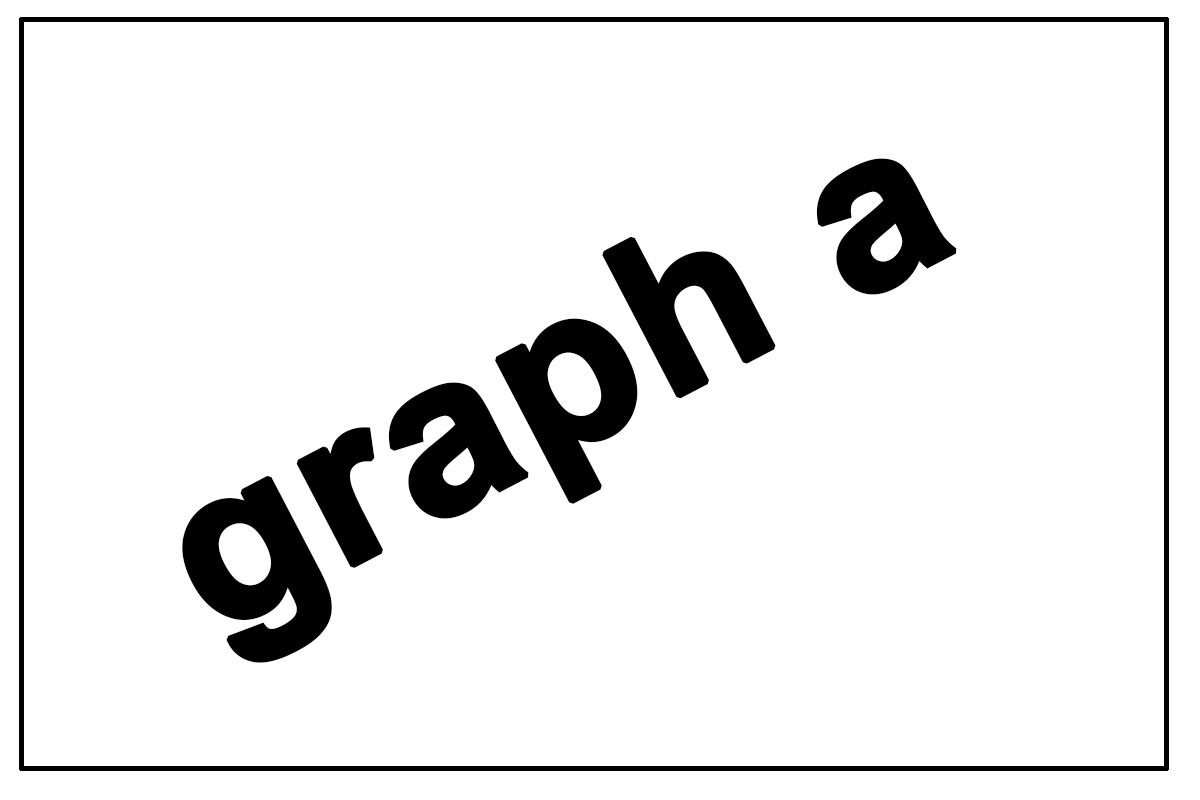
\includegraphics[scale=0.4]{graph_a.png}
	\caption{2D Panorama of the Pellerhaus}
	\label{fig:2d_panorama}
\end{figure}


A 3D Panorama is a two-dimensional image mapped onto a 3d sphere. With such an image it is possible to visualize the complete three dimensional environment from one viewpoint.

\pagestyle{fancy}

\begin{figure}[h]
	\centering
	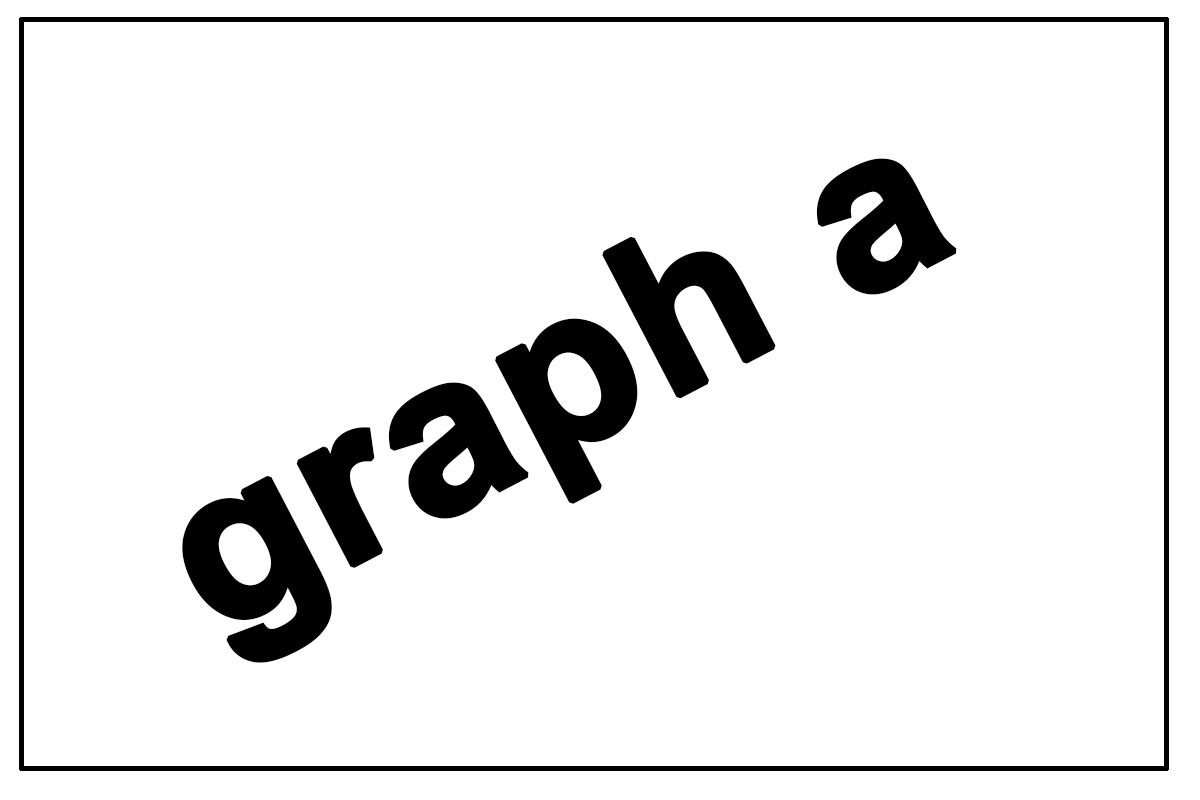
\includegraphics[scale=0.4]{graph_a.png}
	\caption{3D Panorama Sphere}
	\label{fig:3d_panorama_sphere}
\end{figure}

3D Panoramas got a great new use by the introduction of the occulus rift (https://www.oculus.com/). They are used in film production as well, this is a very sophisticated use of integrating a 360 panorama video with virtual 3d objects (http://www.cgmeetup.net/home/google-atap-help-behind-the-scenes/).

There are several types of projections used for 3D panoramas, see \ref{fig:three_projections}.


\section{Types of projections} \label{section_types_of_projections}

Only equirectangular provides a 100 percent coverage! (see \url{http://www.cambridgeincolour.com/tutorials/image-projections.htm})

You can never have perfect "flat" (2d) representations of a sphere. There are always limitations, but you could choose the right projection for your project. More info \url{http://www.progonos.com/furuti/MapProj/Normal/CartDef/MapDef/mapDef.html}

(Houshiar et al. 2015 \parencite{houshiar2015a})

houshiar2015a

\begin{figure}[h]
	\centering
	\begin{subfigure}[b]{0.3\textwidth}
		\centering
		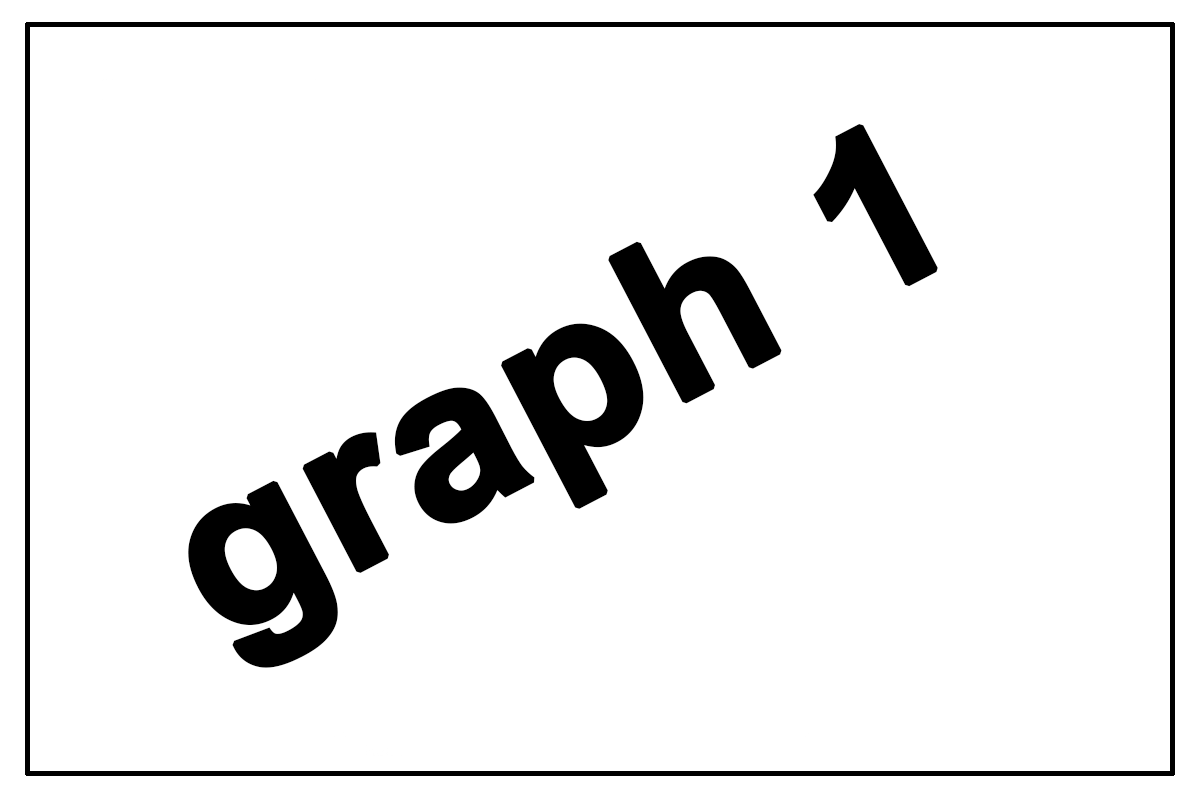
\includegraphics[width=\textwidth]{graph1.png}
		\caption{$Equirectangular$}
		\label{fig:equirectangular}
	\end{subfigure}
	\hfill
	\begin{subfigure}[b]{0.3\textwidth}
		\centering
		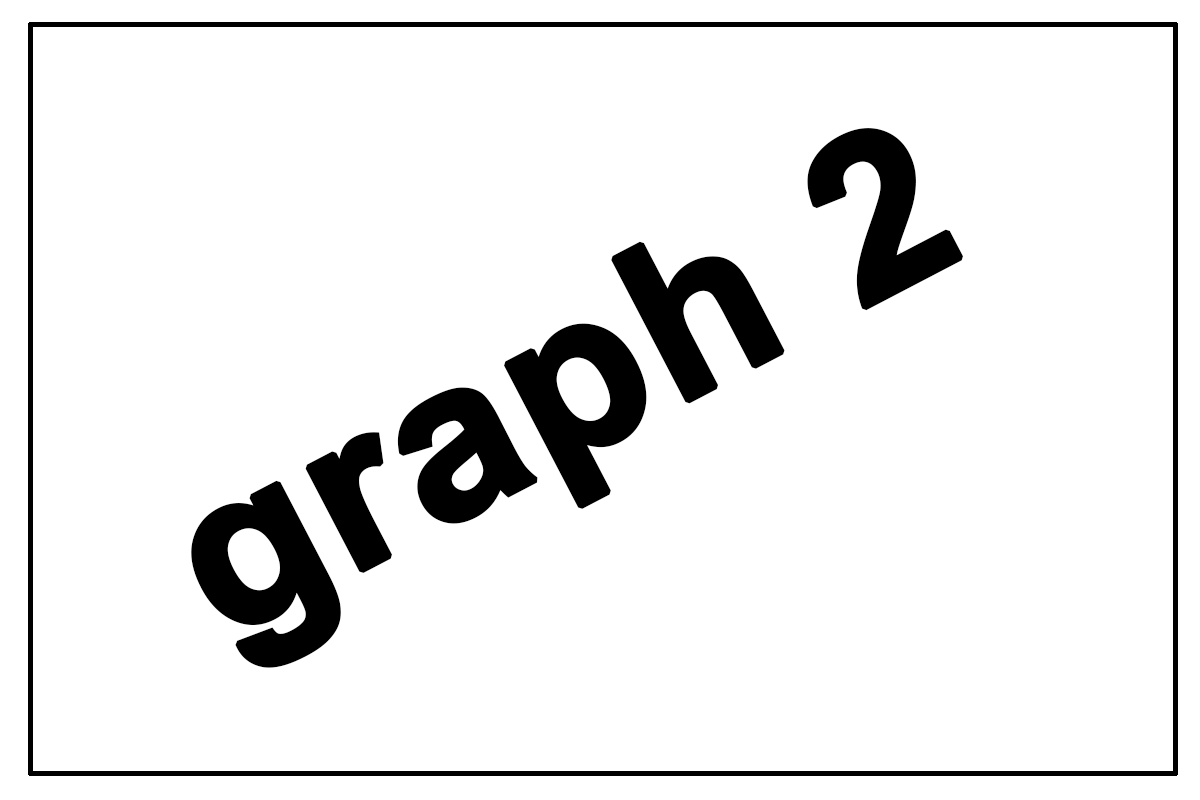
\includegraphics[width=\textwidth]{graph2.png}
		\caption{$Cylindrical$}
		\label{fig:cylindrical}
	\end{subfigure}
	\hfill
	\begin{subfigure}[b]{0.3\textwidth}
		\centering
		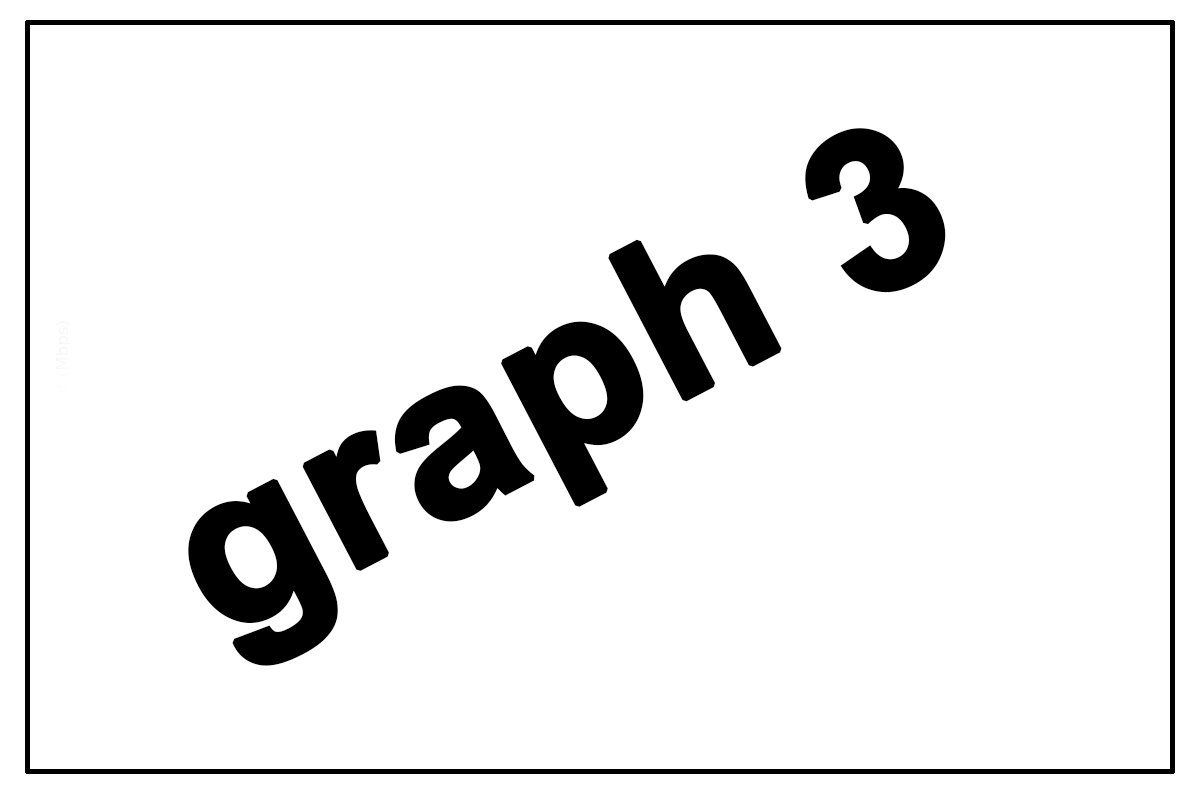
\includegraphics[width=\textwidth]{graph3.png}
		\caption{$Mercator$}
		\label{fig:mercator}
	\end{subfigure}
	\caption{Three example projections}
	\label{fig:three_projections}
\end{figure}

One of the most spread types is the equirectangular projection see \ref{fig:equirectangular}. Due to this reason we will use it primarily in this project.

